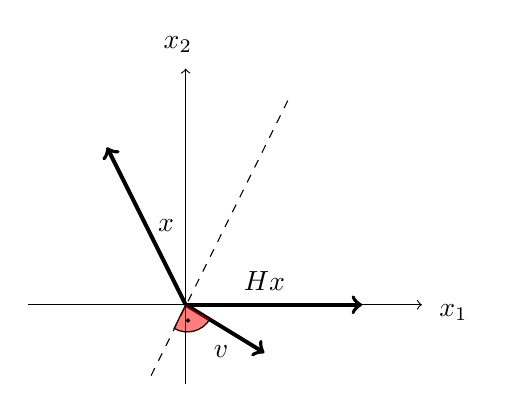
\begin{tikzpicture}

\draw[->] (-2,0) -- (3,0);
\draw[->] (0,-1) -- (0,3);

\draw[->,line width=0.5mm] (0,0) -- (-1,2);
\draw[->,line width=0.5mm] (0,0) -- (2.24,0);

\draw[dashed] (-0.44,-0.9) -- (1.34,2.68);
%\draw[->,line width=0.5mm] (0,0) -- (-0.9, 0.44);
%\draw[->,line width=0.5mm] (0,0) -- (-1,0.61);
\draw[->,line width=0.5mm] (0,0) -- (1,-0.61);



%Rechter Winkel
%\filldraw[red, opacity=0.5] (0,0)--(-0.3375, 0.16) arc (150:244:.375cm) -- (0,0) ;
%\draw[black, opacity=1] (0,0)--(-0.3375, 0.16) arc (150:244:.375cm) -- (0,0) ;

\filldraw[red, opacity=0.5] (0,0)--(-0.1467,-0.3000) arc (240:330:.3339) -- (0,0) ;
\draw[black, opacity=1] (0,0)--(-0.1467,-0.3000) arc (240:330:.3339) -- (0,0) ;
\filldraw(0.03,-0.2) circle (.02cm) ;

%Beschriftung
\draw (3.4,-0.1) node {$x_1$};
\draw (-0.1,3.3) node {$x_2$};

\draw (.45, -.6) node {$v$};
\draw (-.25, 1) node {$x$};
\draw (1,0.3) node {$Hx$};


\end{tikzpicture}